% a mashup of hipstercv, friggeri and twenty cv
% https://www.latextemplates.com/template/twenty-seconds-resumecv
% https://www.latextemplates.com/template/friggeri-resume-cv

\documentclass[lighthipster]{simplehipstercv}
% available options are: darkhipster, lighthipster, pastel, allblack, grey, verylight, withoutsidebar
% withoutsidebar
\usepackage[utf8]{inputenc}
\usepackage[default]{raleway}
\usepackage[margin=1cm, a4paper]{geometry}


%------------------------------------------------------------------ Variablen

\newlength{\rightcolwidth}
\newlength{\leftcolwidth}
\setlength{\leftcolwidth}{0.23\textwidth}
\setlength{\rightcolwidth}{0.75\textwidth}

%------------------------------------------------------------------
\title{New Simple CV}
\author{\LaTeX{} Ninja}
\date{June 2019}

\pagestyle{empty}
\begin{document}


\thispagestyle{empty}
%-------------------------------------------------------------

\section*{Start}

\simpleheader{headercolour}{Mateo}{Hidalgo}{Estudiante}{white}



%------------------------------------------------

% this has to be here so the paracols starts..
\subsection*{}
\vspace{4em}

\setlength{\columnsep}{1.5cm}
\columnratio{0.23}[0.75]
\begin{paracol}{2}
\hbadness5000
%\backgroundcolor{c[1]}[rgb]{1,1,0.8} % cream yellow for column-1 %\backgroundcolor{g}[rgb]{0.8,1,1} % \backgroundcolor{l}[rgb]{0,0,0.7} % dark blue for left margin

\paracolbackgroundoptions

% 0.9,0.9,0.9 -- 0.8,0.8,0.8


\footnotesize
{\setasidefontcolour
\flushright
\begin{center}
    % --- INICIO DEL CÓDIGO PARA LA FOTO ---
    \begin{tikzpicture}
        % 1. Define el borde/márgen del círculo.
        % Ajusta 'radius=2.5cm' para cambiar el tamaño del círculo en la hoja.
        \clip (0,0) circle [radius=2cm];

        % 2. Introduce la imagen y hazle zoom.
        % AJUSTE CRUCIAL: Cambia 'scale=1.5' para hacer zoom IN (agrandar la foto adentro) o OUT.
        % (Prueba valores como 1.8, 2.0, etc. para más zoom).
        \node[inner sep=0pt] at (0,0) {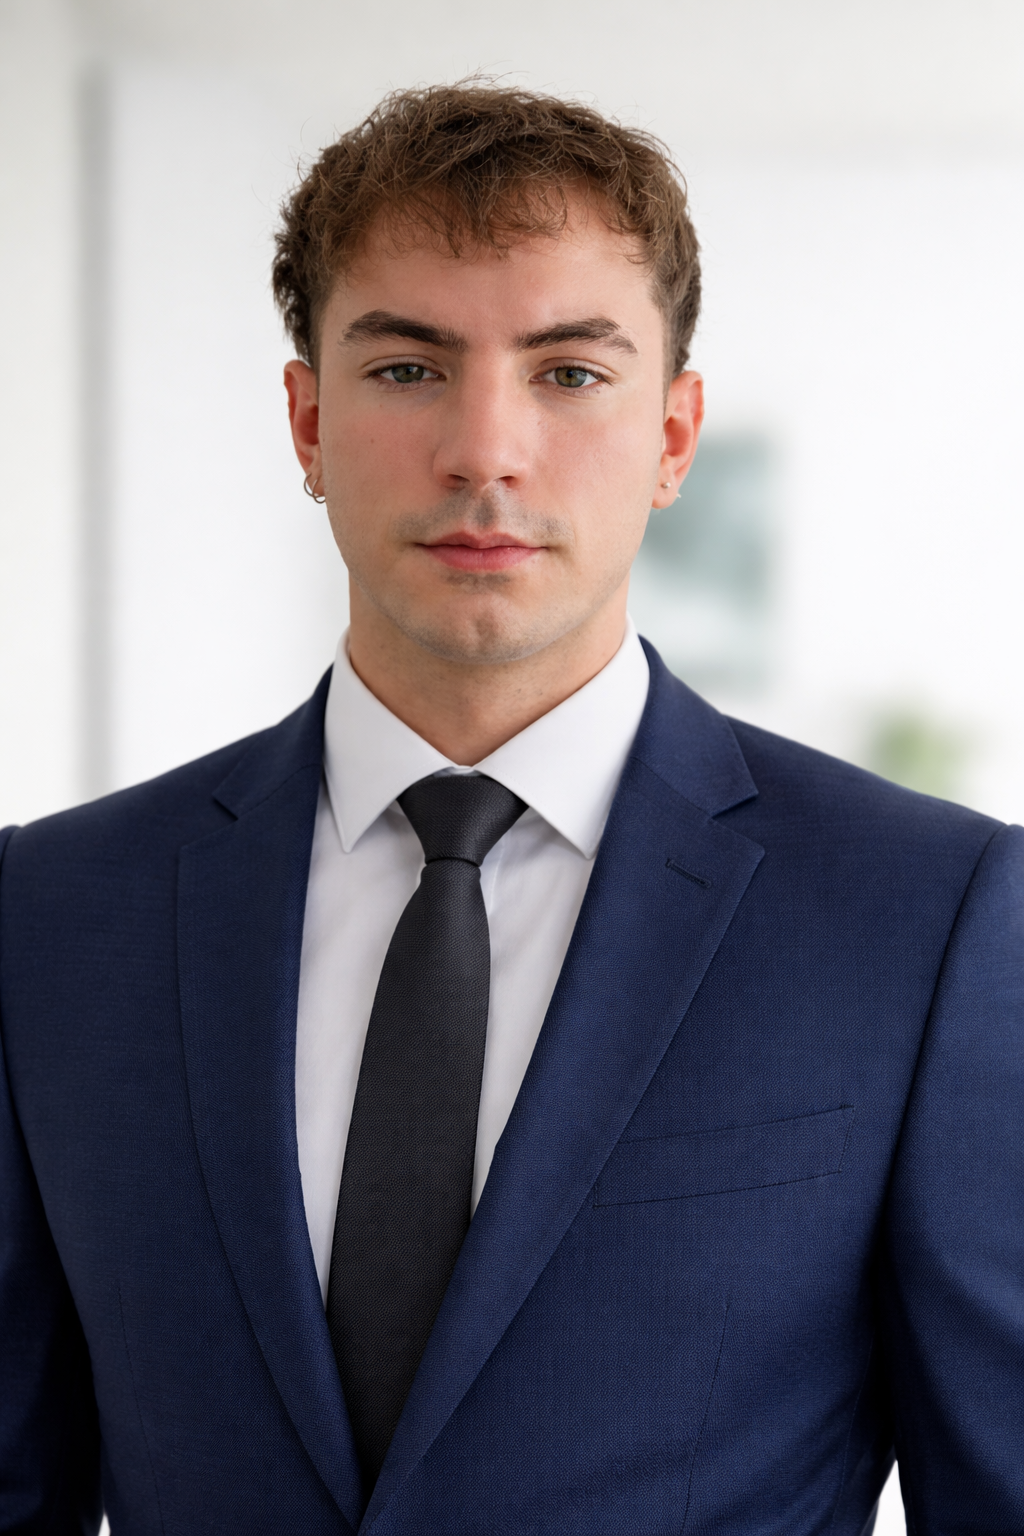
\includegraphics[scale=0.1]{Traje.png}};
    \end{tikzpicture}
    % --- FIN DEL CÓDIGO ---
\end{center}


\bg{cvgreen}{white}{Acerca de mí}\\[0.5em]

{\footnotesize
Soy actualmente estudiante de tercer año de ingeniería industrial en la facultad nacional de cuyo, y emprendendor en negocios gastronómicos}

\bigskip
\bg{cvgreen}{white}{Personal} \\[0.5em]
Mateo Hidalgo

Nacionalidad: Argentina

2005

\bigskip

\bg{cvgreen}{white}{Areas de especialización} \\[0.5em]

Matemáticas ~•~ Física ~•~ Automatización ~•~ Liderazgo

\bigskip




\bigskip

\bg{cvgreen}{white}{Interests}\\[0.5em]

\texttt{Emprendedurismo} ~/~ \texttt{Ingeniería}

\texttt{Computación} ~/~ \texttt{Empresas} ~/~ \texttt{Python}


\vspace{4em}


\infobubble{\faTwitter}{cvgreen}{white}{@MJHidalgo}
\infobubble{\faFacebook}{cvgreen}{white}{Mateo Hidalgo}
\infobubble{\faGithub}{cvgreen}{white}{MHidalgo}

\phantom{turn the page}

\phantom{turn the page}
}
%-----------------------------------------------------------
\switchcolumn

\small
\section*{Pequeño Resumen}

\begin{tabular}{r| p{0.5\textwidth} c}
    \cvevent{2021--2023}{Asistente de producción de eventos}{Asistente}{Ricky Videla \color{cvred}}{Asistente en la realización de la producción de eventos a gran escala de casamientos, cumpleaños y diversos festejos de la mano del importante productor Ricky Videla en Mendoza}{Ricky.jpg} \\
\end{tabular}
\vspace{3em}

\begin{minipage}[t]{0.35\textwidth}
\section*{Titulos}
\begin{tabular}{r p{0.6\textwidth} c}
    \cvdegree{1710}{Secundario}{Certificado}{Instituto Murialdo \color{headerblue}}{}{Murialdo.jpg} \\
    \cvdegree{1711}{Introducción a la programación con Python}{Certificado}{Santander Open Acadedemy \color{headerblue}}{}{Santander-Emblema.png}\\
\end{tabular}
\end{minipage}\hfill
\begin{minipage}[t]{0.3\textwidth}
\section*{Programación}
\begin{tabular}{r @{\hspace{0.5em}}l}
     \bg{skilllabelcolour}{iconcolour}{html, css} &  \barrule{0.3}{0.5em}{cvpurple}\\
     \bg{skilllabelcolour}{iconcolour}{\LaTeX} & \barrule{0.25}{0.5em}{cvgreen} \\
     \bg{skilllabelcolour}{iconcolour}{python} & \barrule{0.45}{0.5em}{cvpurple} \\
\end{tabular}
\end{minipage}




\bigskip

\section*{Languajes}
\begin{tabular}{l | ll}
\textbf{Spanish} &  & {\phantom{x}\footnotesize Lengua materna} \\
\textbf{English} & B2 & \pictofraction{\faCircle}{cvgreen}{3}{black!30}{2}{\tiny} \\
\end{tabular}
\bigskip










\end{paracol}


\vspace*{\fill} 

%----------------------------------------------------------------------------------------
%	FINAL FOOTER
%----------------------------------------------------------------------------------------
\begin{center}
    \fontfamily{\sfdefault}\selectfont \color{black!70} \small
    Mateo Hidalgo \icon{\faEnvelopeO}{cvgreen}{} Argentina \icon{\faMapMarker}{cvgreen}{} Mendoza \icon{\faPhone}{cvgreen}{}+54 261 500-1317 \\[0.5em]
    \icon{\faAt}{cvgreen}{} \protect\url{MateoHidalgo.com}
\end{center}

\end{document}
